\chapter{Rotation}

\section*{LEARNING OUTCOMES}
{
\begin{center}
\fcolorbox{black}{shadecolor}
{%
    \parbox{0.95\textwidth}
    {%
        \small
        {
        \begin{itemize}
            \item Describe the concept of rotational motion to the students.
            \item Differentiate rotational motion from linear and circular motion.
            \item Introduce different instruments to measure rotational speed.
        \end{itemize}
        }
    }%
}
\end{center}
}

\section*{DEMONSTRATIONS}
\section*{Tachometer}
Tachometer is a device used to measure the rate of rotation. It counts the number of rotations made by an object in a specific interval of time and calculates the rate of rotation.

To build a tachometer, you will need:
\begin{table}[H]
    \centering
    \begin{tabular}{|c|l|c|}\hline
    1   &   10 k$\Omega$ potentiometer  &   1\\\hline
    2   &   470 $\Omega$ resistor       &   1\\\hline
    3   &   Push button                 &   1\\\hline
    4   &   Box (for assembling the tachometer)            &   1\\\hline
    5   &   DC motor                    &   1\\\hline
    6   &   L298N: Motor driver         &   1\\\hline
    7   &   IR transmitter              &   1\\\hline
    8   &   IR receiver                 &   1\\\hline 
    9   &   Arduino UNO                 &   1\\\hline
    10  &   Connecting wires            &   -\\\hline
    \end{tabular}
\end{table}

\subsection*{Connections}
\begin{enumerate}[leftmargin=*]
    \item Connect one end of the 470 $\Omega$ resistor with the anode of IR transmitter and its other end with 5V pin. Connect the cathode of IR transmitter with GND of Arduino.
    \item Connect one end of the 10 k$\Omega$ resistor with the cathode of IR receiver  and connect its other end with GND of Arduino. Connect the anode of IR receiver with 5V pin of Arduino.
    \item Connect the junction of IR receiver and 10 k$\Omega$ resistor with pin A5 of Arduino. 
    \item Connect 12 V power supply to the motor driver through a push button. Also connect GND of Arduino with GND of motor driver. 
    \item Connect two control pins of the motor driver to 5V and GND of Arduino.
    \item Connect the output pins of the motor driver with the outer terminals of the potentiometer. 
    \item Connect the middle pin of the potentiometer with any terminal of DC motor.
    \item Connect the remaining terminal of the DC motor with GND of the motor driver.
\end{enumerate}

	\begin{figure}[H]
	\centering 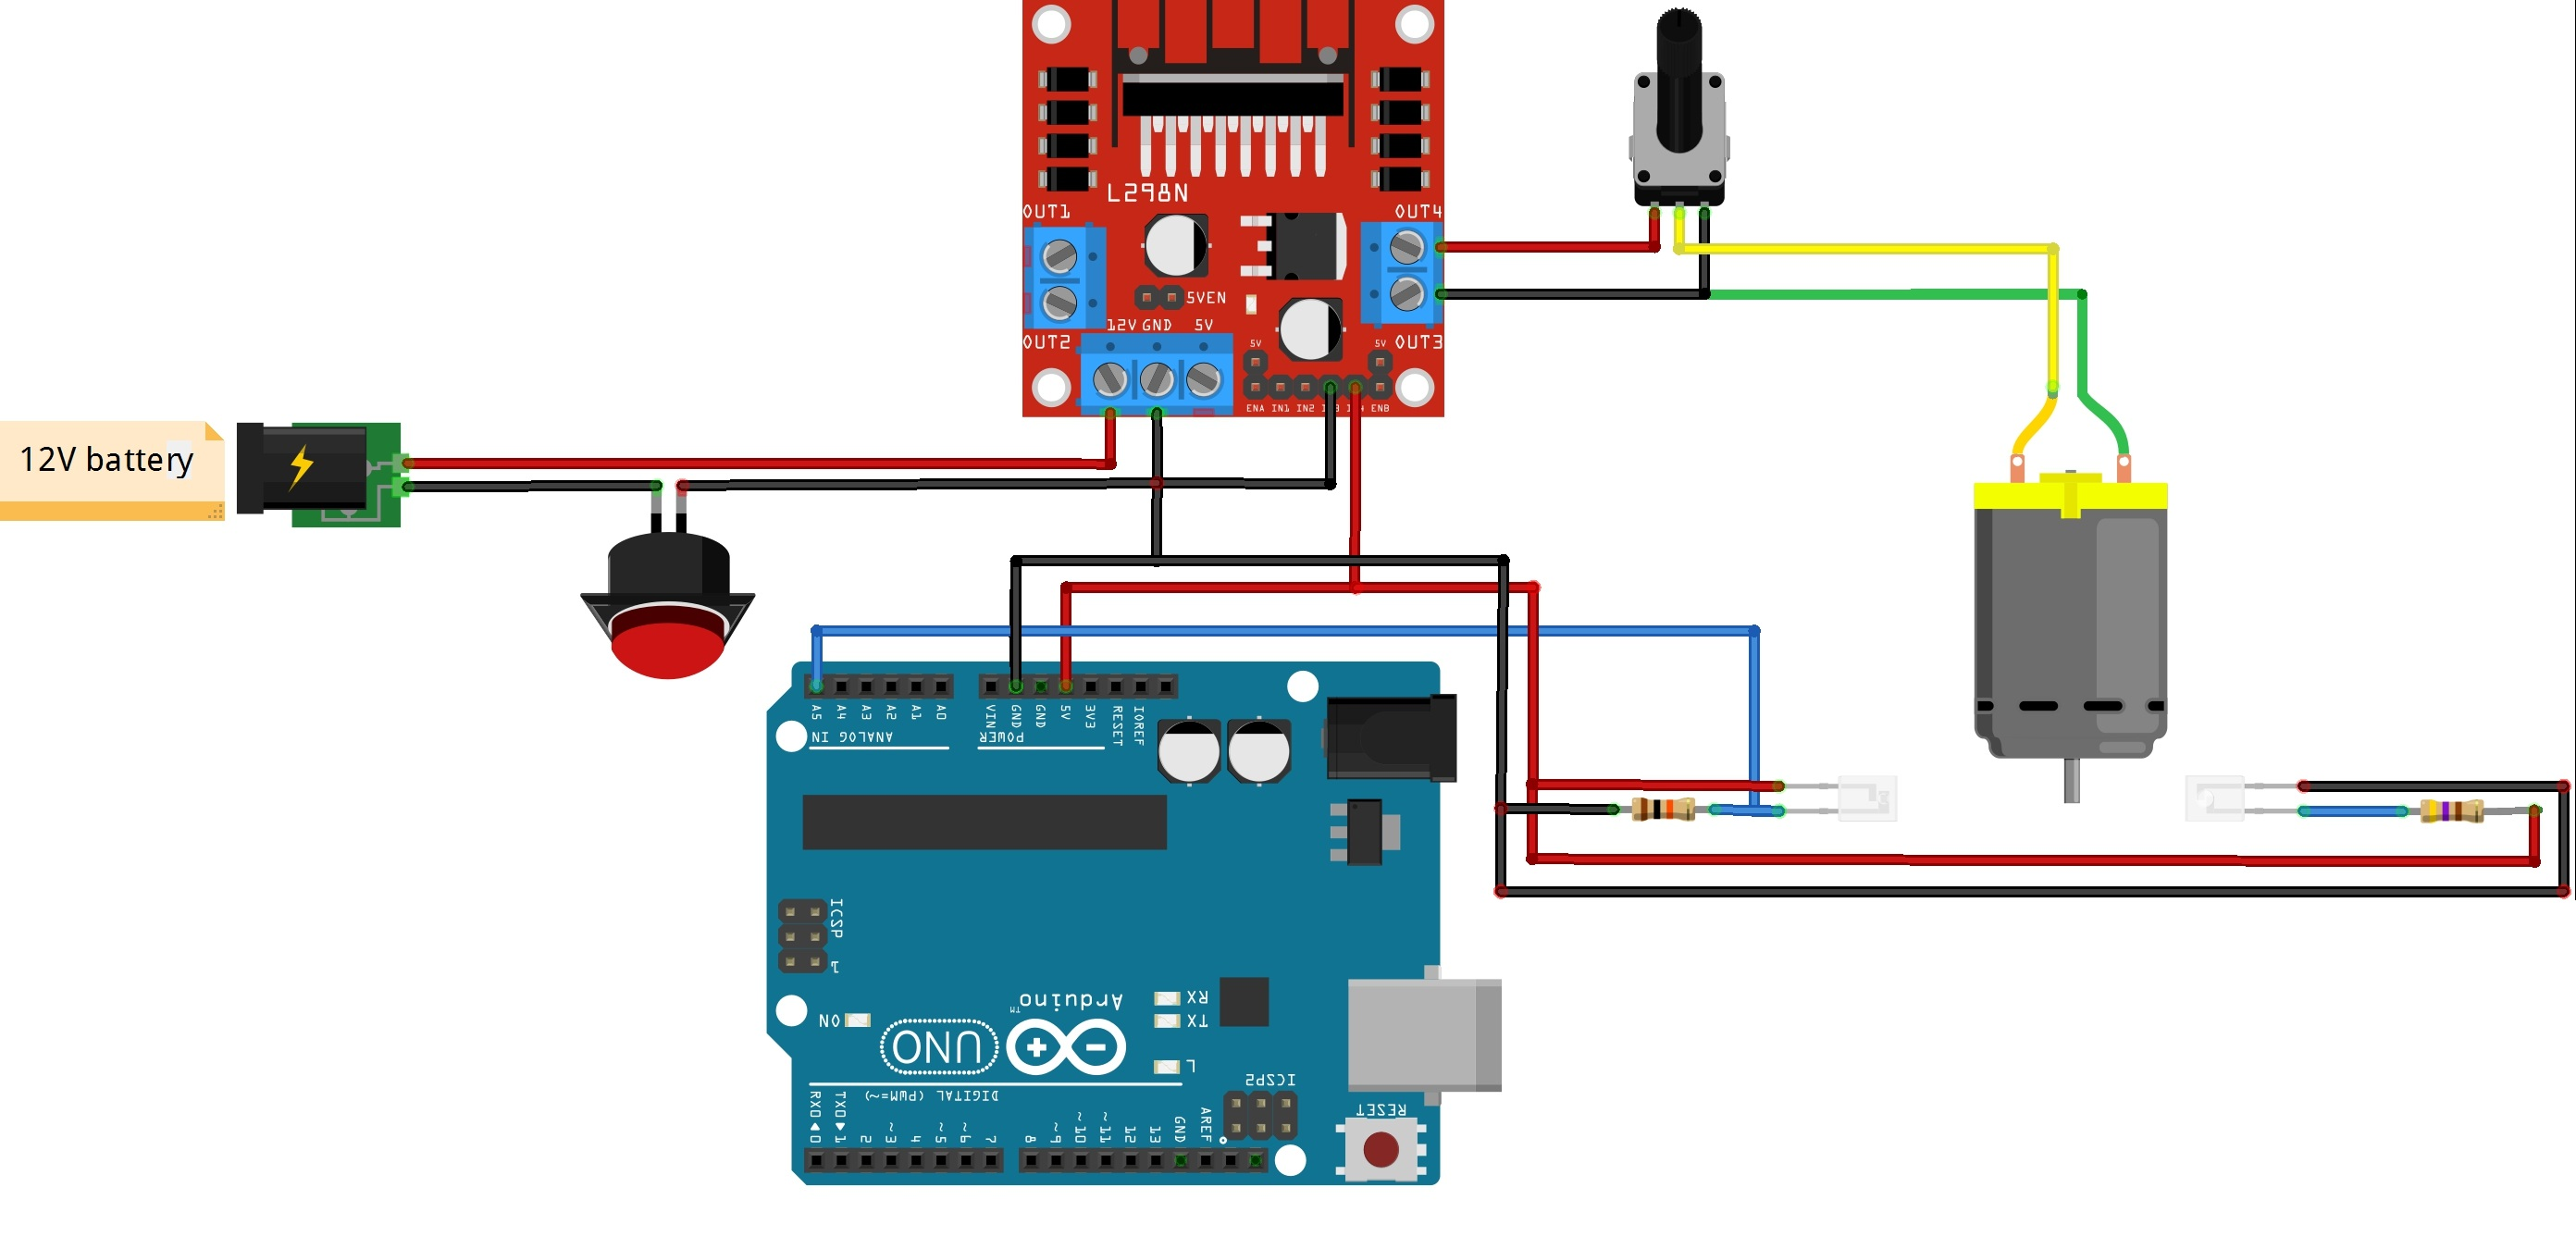
\includegraphics[width=0.7\linewidth]{tachometer.jpg}
	\caption{Circuit diagram}
	\end{figure}

\subsection*{Procedure}
\begin{enumerate}[leftmargin=*]
     \item Copy lst. \ref{lst:rot} to a new Arduino sketchbook. Upload the code to your Arduino board. Also open the Serial Monitor.
    \item Turn the switch ON to supply the power to the motor.
    \item Rotate the knob of the potentiometer to adjust the speed of the motor. Note the reading on the Serial Monitor.
    \item Repeat the experiment by varying the speed of the motor.
\end{enumerate}

\begin{lstlisting}[language=Arduino, numbers=none, caption={Arduino code for measuring the speed of a moving object},captionpos=b, label={lst:rot}]

int i r = A5, x, y, yold, rps ,rpm;
unsigned long time;
unsigned long previousMillis =0;
void setup () 
{
    // put your setup code here, to run once:
    Serial.begin (9600);
    pinMode (ir, INPUT);
    yold = 0;
    rps = 0;
}

void loop ()
{
    // put your main code here, to run repeatedly :
    unsigned long currentMillis = millis () ;
    x = analogRead (ir) ;
    if (x >= 1015)
    { 
        // calibrating IR sensor
        y = 1;
    }
    else
    {
        y = 0;
        yold = 0;
    }

    time = currentMillis - previousMillis ;
    
    if ( time <= 5000)
    {
        if (y > yold )
        {
            rps = rps+y ;
            yold = y ;
        }
    }
    else
    {
        rpm = rps *12;
        Serial.print ( millis () /1000) ;
        Serial.print ( \`\t’ ) ;
        Serial.println (rpm) ;
        previousMillis = currentMillis ;
        rps = 0;
    }
}


\end{lstlisting}

\subsection*{Additional Notes}
\begin{itemize}[noitemsep, leftmargin=*]
    \item The measured RPM can be calibrated by using another tachometer. For this purpose, run the motor with the 5V supply of Arduino and measure the rotational speed of the motor. Calibrate the RPM reading of the code accordingly.
\end{itemize}

\subsection*{Precautions}
\begin{itemize}[noitemsep, leftmargin=*]
    \item Do not power the motor directly with the Arduino board. Always use a motor driver.
    \item The motor may wear out due to excessive use and may need replacement. 
\end{itemize}

\begin{figure}[H]
    \centering
    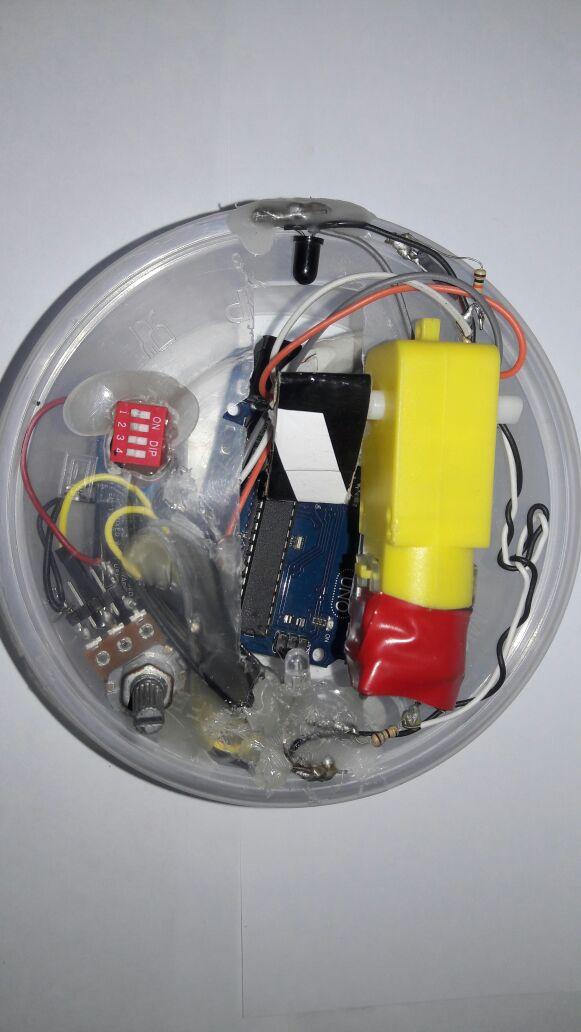
\includegraphics[scale=0.20]{Figures/rot-hardware.jpg}
    \caption{Hardware of the speedometer}
    \end{figure}
    

